\documentclass[a4paper,10pt]{report}
\usepackage[utf8]{inputenc}
\usepackage{graphicx}
\usepackage{verbatim}
\usepackage{ctable} % for \specialrule command

%\usepackage[a4paper, total={6in, 8in}]{geometry}
% Title Page
\title{\textbf{OPTICAL COMMUNICATION COMPONENTS \\ Lab 7}}
\author{Nicola Simoni, Tadewos Somano, Melkamsew Tenaw}
\date{University of Brescia, Faculty of Engineering\\A.Y. 2013-2014}


\begin{document}
\maketitle


%%%%%%%%%%%%%%%%%%%%%%%%%%%%%%%%%%%%%%%%%%%%%%%%%%%%%%%%%%%%%%%%%%%%%%%%%%%%%%%%%%%%%%%%%%%%%
\section*{Question 1}
We have a loop structure that represents a transmission link consisting of several identical spans of fiber, with an
amplifier to compensate for the fiber attenuation at each loop.
Non linear and dispersive effects of the optical fiber are turned off. Setup parameters simulate a transmission link
that is 4000 Km long. The link is divided into 40 spans of 100 Km length each.

We want to know what should be the gain of the optical amplifier in order to fully compensate for the fiber loss
within each span.
Given that the fiber has an attenuation $\alpha$ [dB/Km], the attenuation of each span is equal to
$\alpha_{span}=100 \cdot \alpha$ dB. Then the gain of the amplifier G has to be equal to the value in decibel introduced
by the attenuation. For example, if the attenuation of the 100 Km span is equal to $\alpha_{span}=20$ dB,
then the gain of the amplifier has to be equal to G=20 dB.

In fact the power budget of the span can be computed as:
$$P_{out} \ [dBm]=P_{in} \ [dBm]-\alpha_{span} \ [dB]+G \ [dB]=P_{in} \ [dBm]$$

%%%%%%%%%%%%%%%%%%%%%%%%%%%%%%%%%%%%%%%%%%%%%%%%%%%%%%%%%%%%%%%%%%%%%%%%%%%%%%%%%%%%%%%%%%%%%
\section*{Question 2}
The noise figure of each optical amplifier is initially set at 3 dB.
This parameter is defined as: $$F=10 \ log \left( \frac{SNR_{in}}{SNR_{out}} \right)$$
where $SNR_{out}$ and $SNR_{in}$ are the signal-to-noise ratios measured at the output and at the input of the amplifier, respectively.
\\This means that: $$SNR_{out} \ [dB]=SNR_{in} \ [dB]-F \ [dB]$$
that is, at the output of the device the signal-to-noise ratio is degraded by the noise figure, that in our case is 3 dB.

%%%%%%%%%%%%%%%%%%%%%%%%%%%%%%%%%%%%%%%%%%%%%%%%%%%%%%%%%%%%%%%%%%%%%%%%%%%%%%%%%%%%%%%%%%%%%
\section*{Question 3}
We run the simulation, in Figure \ref{3_1} is shown the eye diagram after each loop. As we can notice the eye is open, the BER is
$\approx 10^{-11}$, so the transmitted data are fully recovered at the receiver.

\begin{figure}[!ht]
   \centering
   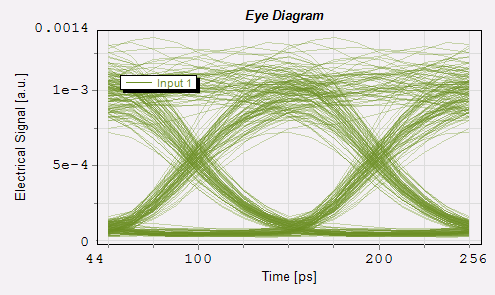
\includegraphics[width=11cm]{3_1.png}\\
   \caption{Eye diagram F=3 dB.}
   \label{3_1}
 \end{figure}

Actually the noise figure of a real optical amplifier is from 4.5 to 6 dB. So we set the noise figure to 6 dB and we run the simulation again.
The BER now is $\approx 4.594 \cdot 10^{-6}$, that is five orders of magnitude bigger, respect to the previous case.
The BER is worse, respect to the case with F=3 dB, because the noise figure is higher, and this translates into an increasing of the
noise at the output of the amplifier.
In Figure \ref{3_2} is shown the eye diagram: we can observe that now the eye is more closed and it is difficult to discriminate the two levels.

\begin{figure}[!ht]
   \centering
   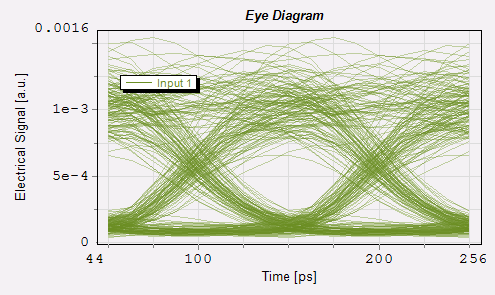
\includegraphics[width=11cm]{3_2.png}\\
   \caption{Eye diagram F=6 dB.}
   \label{3_2}
 \end{figure}
 
 \newpage
 In Figure \ref{3_wform} is shown the waveform of the signal: we can notice the signal takes also intermediate values, respect to the values
 that correspond to ``0'' and ``1''.
 
 \begin{figure}[!ht]
   \centering
   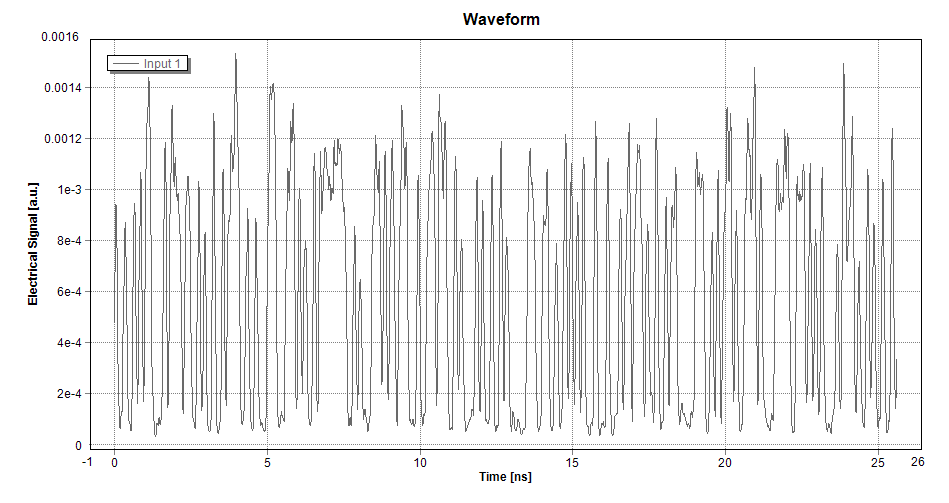
\includegraphics[width=11cm]{3_wform.png}\\
   \caption{Waveform F=6 dB.}
   \label{3_wform}
 \end{figure}

 In Figure \ref{3_1spec} and \ref{3_2spec} are represented the optical power levels of the signals obtained with F=3 and F=6 dB respectively.
 
 \newpage
 \begin{figure}[!ht]
   \centering
   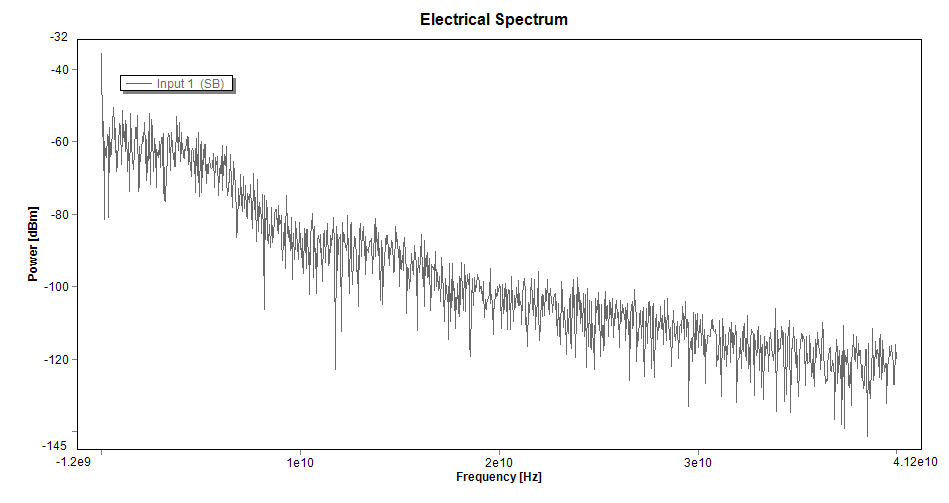
\includegraphics[width=11cm]{3_1pw.png}\\
   \caption{Spectrum F=3 dB.}
   \label{3_1spec}
 \end{figure}
 
  \begin{figure}[!ht]
   \centering
   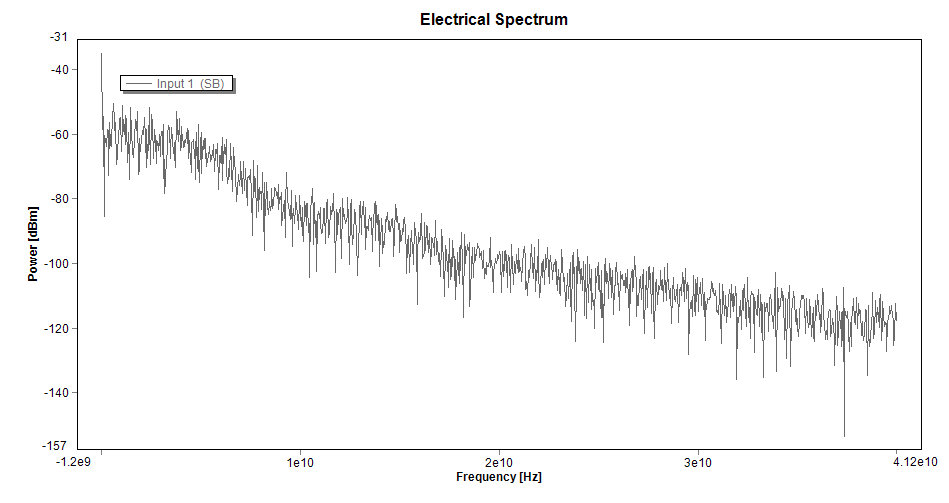
\includegraphics[width=11cm]{3_2pw.png}\\
   \caption{Spectrum F=6 dB.}
   \label{3_2spec}
 \end{figure}
 
 
 
 
 \newpage
%%%%%%%%%%%%%%%%%%%%%%%%%%%%%%%%%%%%%%%%%%%%%%%%%%%%%%%%%%%%%%%%%%%%%%%%%%%%%%%%%%%%%%%%%%%%%
\section*{Exercise 1}
We vary the noise figure from 3 to 6 dB, in steps of 1 dB, and we measure the relative BER. The simulation is relative to the 4000 Km length link.
In Figure \ref{es1} is shown the result.

 \begin{figure}[!ht]
   \centering
   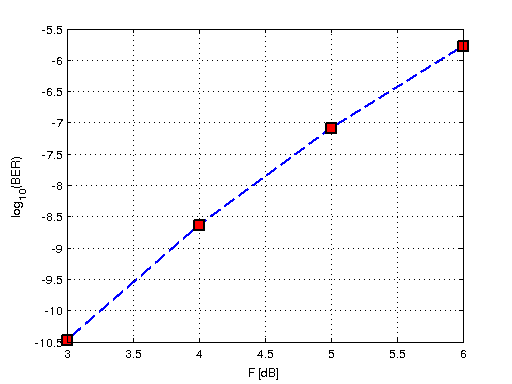
\includegraphics[width=11cm]{es1.png}\\
   \caption{BER versus F.}
   \label{es1}
 \end{figure}

we consider the BER acceptable when it is smaller than $10^{-9}$, that is $< -9$ in logarithmic scale.
To find the limit value of the noise figure for which we have acceptable BER, we zoom the graph: the noise figure must be smaller than
3.8 dB, as shown in Figure \ref{es1_2}.

\begin{figure}[!ht]
   \centering
   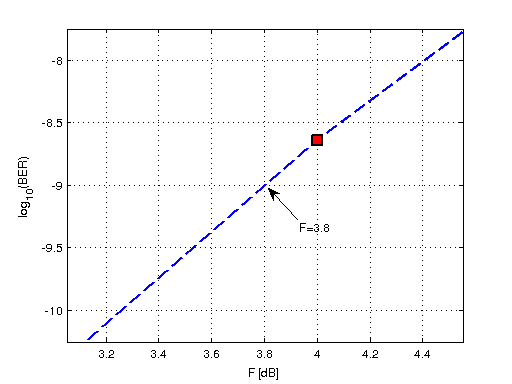
\includegraphics[width=11cm]{es1_2.png}\\
   \caption{BER versus F, limit value.}
   \label{es1_2}
 \end{figure}


\newpage
%%%%%%%%%%%%%%%%%%%%%%%%%%%%%%%%%%%%%%%%%%%%%%%%%%%%%%%%%%%%%%%%%%%%%%%%%%%%%%%%%%%%%%%%%%%%%
\section*{Exercise 2}
We set the noise figure to 6 dB. We take measures of the BER for different fiber lengths by reducing the number of fiber spans.
We use a step of 5 loops, that corresponds to 500 Km: the length is computed as $L=L_{tot}/n^\circ \ loops$.
In Figure \ref{es2} is shown the result. To better represent the curve, both axes are in logarithmic scale.
By zooming the graph, we can notice that we have acceptable BER for a value of spatial coordinate less than 4.93,
that in linear scale is nearly 85100 m.

\begin{figure}[!ht]
   \centering
   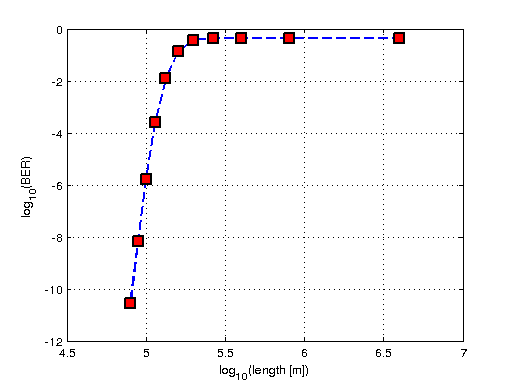
\includegraphics[width=11cm]{es2.png}\\
   \caption{BER versus length, F=6 dB.}
   \label{es2}
\end{figure}

%%%%%%%%%%%%%%%%%%%%%%%%%%%%%%%%%%%%%%%%%%%%%%%%%%%%%%%%%%%%%%%%%%%%%%%%%%%%%%%%%%%%%%%%%%%%%
\section*{Exercise 3}
We set the noise figure to 4.5 dB and we repeat the simulation as in Exercise 2.
By reading on the graph, the acceptable BER is for a value of spatial coordinate less than 4.98, that in linear scale is nearly 95500 m.
As now the noise figure is lower, we can reach a farther distance (at parity of BER), respect to the case with F=6 dB.

\begin{figure}[!ht]
   \centering
   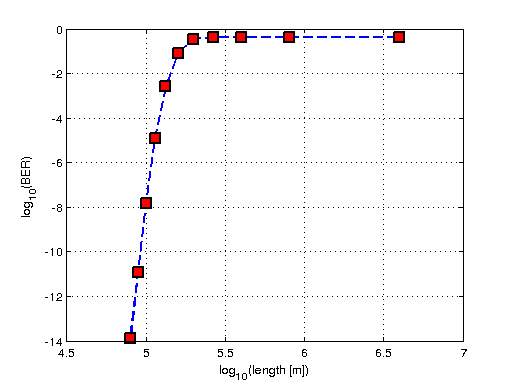
\includegraphics[width=11cm]{es3.png}\\
   \caption{BER versus length, F=4.5 dB.}
   \label{es3}
\end{figure}


\newpage
%%%%%%%%%%%%%%%%%%%%%%%%%%%%%%%%%%%%%%%%%%%%%%%%%%%%%%%%%%%%%%%%%%%%%%%%%%%%%%%%%%%%%%%%%%%%%
\section*{Question 4}
Now we study the case in which we want to reduce costs, and so we use the less possible number of amplifiers.
By doing so, we necessarily have to increase the gain.
 We reduce the value of the setting ``loop'' from 40 to 20, in this way the number of amplifiers used is halved.
 The length of each span fiber is increased from 100 Km to 200 Km and the gain of the amplifier is increased from 20 dB to 40 dB.
 The noise figure is set at 3 dB.
 We run the simulation: in Figure \ref{es41} and \ref{es42} are shown the optical spectrum and the eye diagram.
 The eye diagram shows that the signal is very degraded, the BER is $\approx 0.29$, that is too far to be acceptable.
Even if the noise figure is low the received signal is bad. This is due to the fact that, by halving the number of amplifiers,
the signal on each span is doubly attenuated before being amplified. Before reaching the amplifier the signal is small
and its power is comparable with the power of the noise introduced by the photo-detector.
So the amplifiers will amplify a very noisy signal.

\begin{figure}[!ht]
   \centering
   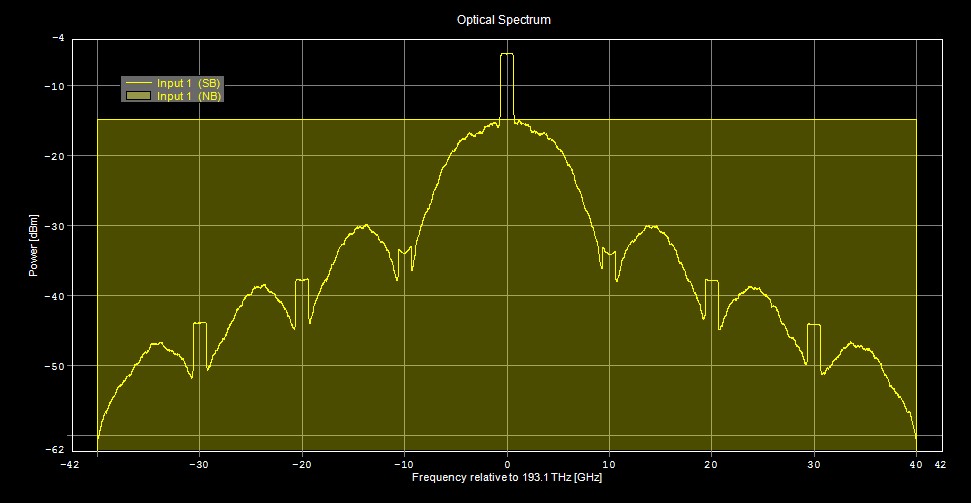
\includegraphics[width=11cm]{es41.png}\\
   \caption{Optical spectrum.}
   \label{es41}
\end{figure}


\begin{figure}[!ht]
   \centering
   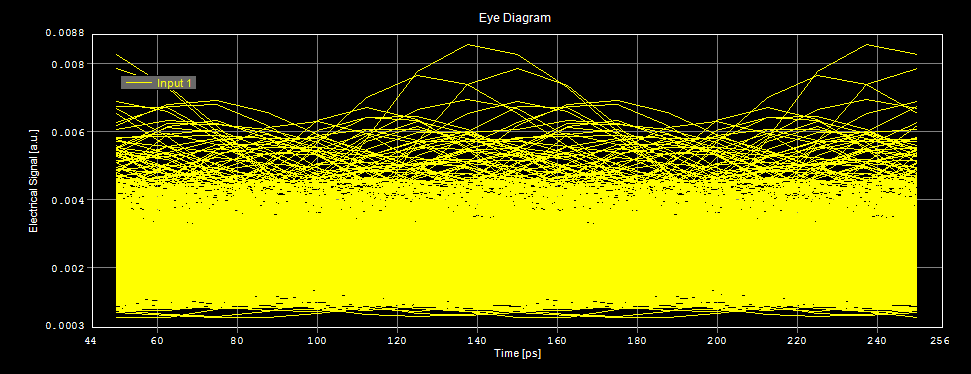
\includegraphics[width=11cm]{es42.png}\\
   \caption{Eye diagram.}
   \label{es42}
\end{figure}

\newpage
%%%%%%%%%%%%%%%%%%%%%%%%%%%%%%%%%%%%%%%%%%%%%%%%%%%%%%%%%%%%%%%%%%%%%%%%%%%%%%%%%%%%%%%%%%%%%
\section*{Question 5}
There is a limit on the noise figure that an amplifier can reach. In fact, for high gain amplifiers, we could write the following
expression of the noise figure:
$$F=10 \ log \left( \frac{SNR_{in}}{SNR_{out}} \right)=10 \ log \left( \frac{2 n_{sp} (G-1) +1}{G} \right)$$
where $n_{sp}=N_e/(N_e-N_g)$ is the spontaneous emission factor. For amplifiers with high inversion $n_{sp} \rightarrow 1$ and so:
$$F \approx 10 \ log \left( \frac{2 n_{sp} G}{G} \right)=3 \ dB$$
Optical amplifiers with higher gain then have lower noise figure, even if the lowest limit possible is $F \approx 3$ dB.


%%%%%%%%%%%%%%%%%%%%%%%%%%%%%%%%%%%%%%%%%%%%%%%%%%%%%%%%%%%%%%%%%%%%%%%%%%%%%%%%%%%%%%%%%%%%%
\section*{Exercise 4}
Now we investigate the dependence of BER on the number of amplifier used in the link: we fix the noise figure to 4.5 dB and we vary
the parameter ``loops''. In this way we automatically vary the number of amplifiers used.
In Figure \ref{4amplifiers} is shown the result. From the graph we can conclude that, to have an acceptable BER, we need to use
at least 43 amplifiers.

\begin{figure}[!ht]
   \centering
   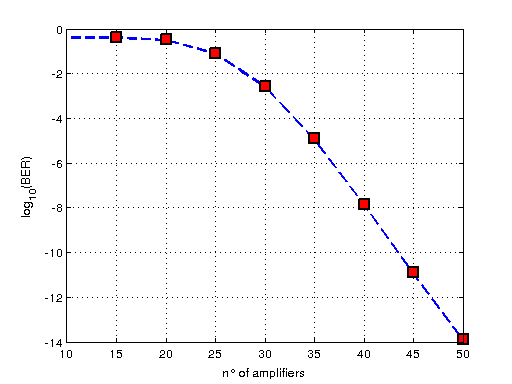
\includegraphics[width=11cm]{4amplifiers.png}\\
   \caption{BER versus n$^\circ$ amplifiers.}
   \label{4amplifiers}
\end{figure}

The total link length was 4000 Km, that divided into 43 spans, means that one span is nearly 93 Km long.
So the maximum fiber span length is 93 Km. If the fiber attenuation is $\alpha$ [dB/Km], the attenuation introduced by each span
is equal to $\alpha_{span}=93 \cdot \alpha$ dB. If we take $\alpha= 0.2$ [dB/Km], then $\alpha_{span} \approx 18.6$ dB.
So to compensate for the span attenuation, the amplifiers must have a gain of at least $G=18.6$ dB.

%%%%%%%%%%%%%%%%%%%%%%%%%%%%%%%%%%%%%%%%%%%%%%%%%%%%%%%%%%%%%%%%%%%%%%%%%%%%%%%%%%%%%%%%%%%%%
\section*{Question 6}
Now we will investigate the limitations imposed on WDM systems due to the non-flat shape of amplifier gain versus wavelength.
We multiplex signals at eight wavelengths and we transmit them through many amplified fiber spans, by the means of a loop.
We set the parameter ``loops'' to 1 and we run the simulation. The input powers of the eight channels are initially all equal.
At the end of the simulation, instead, the powers are different. In Figure \ref{es6} is shown the optical spectrum at the end
of the fiber.

\begin{figure}[!ht]
   \centering
   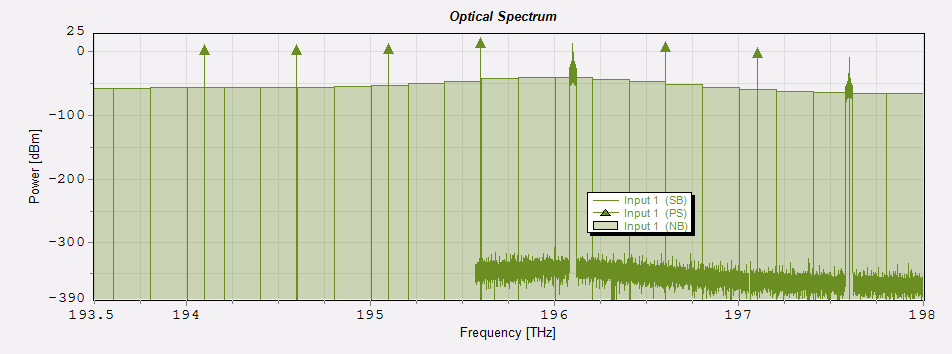
\includegraphics[width=12cm]{es6.png}\\
   \caption{Optical spectrum.}
   \label{es6}
\end{figure}

The received powers are reported in Table \ref{tab}. The difference in power level between the strongest and the weakest channel
(channel 5 and 8 respectively) is 16.942-(-6.255) dBm = 23.197 dBm.

\begin{table}[ht!]
  \begin{center}
    \begin{tabular}{|c|c|}
      \specialrule{.1em}{.05em}{.05em}
	 Frequency [THz] & Power [dBm]\\

	\hline
	194.1 & 3.232\\
	\hline
	194.6 & 3.398\\
	\hline
	195.1 & 5.687\\
	\hline
	195.6 & 14.530\\
	\hline
	196.1 & 16.942\\
	\hline
	196.6 & 8.829\\
	\hline
	197.1 & -0.755\\
	\hline
	197.6 & -6.255\\
	
      \specialrule{.1em}{.05em}{.05em}
    \end{tabular}
  \end{center}
\caption{Peak powers.}
\label{tab}
\end{table}

In Figure \ref{es6scope1} and \ref{es6scope2} are shown the scope traces of the channels 5 and 8.
We can notice that the maximum amplitude of channel 5 is nearly 0.12, while for channel 8 is nearly 0.0005.
This means that the second is about 240 times weaker: the value $10 \cdot \log_{10}(240) \approx 23 \ dBm$ corresponds
in fact to the difference of power in dBm between the two channels.

\begin{figure}[!ht]
   \centering
   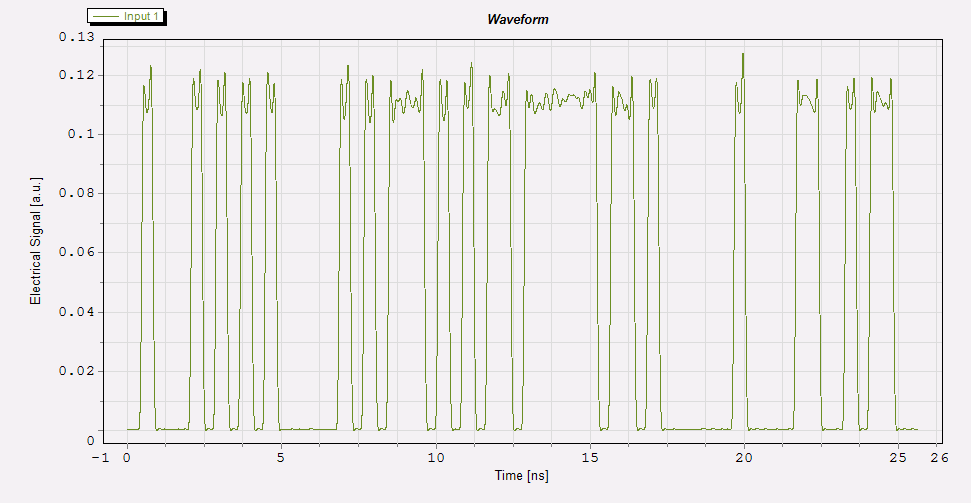
\includegraphics[width=11cm]{es6scope1.png}\\
   \caption{Scope, channel 5.}
   \label{es6scope1}
\end{figure}

\begin{figure}[!ht]
   \centering
   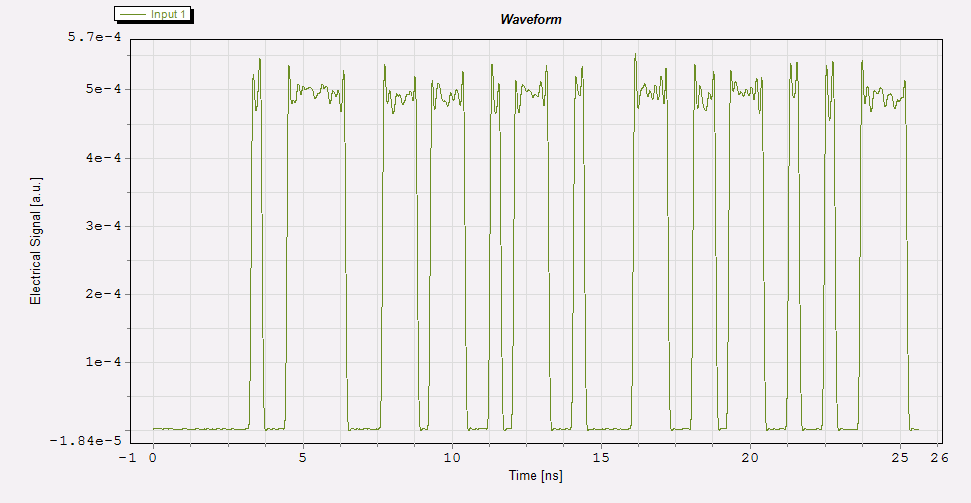
\includegraphics[width=11cm]{es6scope2.png}\\
   \caption{Scope, channel 6.}
   \label{es6scope2}
\end{figure}


%%%%%%%%%%%%%%%%%%%%%%%%%%%%%%%%%%%%%%%%%%%%%%%%%%%%%%%%%%%%%%%%%%%%%%%%%%%%%%%%%%%%%%%%%%%%%
\section*{Question 7}
We set the number of loops to 5 and we run the simulation again: this is equivalent to a transmission through a link with
5 amplified fiber spans. In Figure \ref{es7} is shown the spectrum at the end of the fiber.

\begin{figure}[!ht]
   \centering
   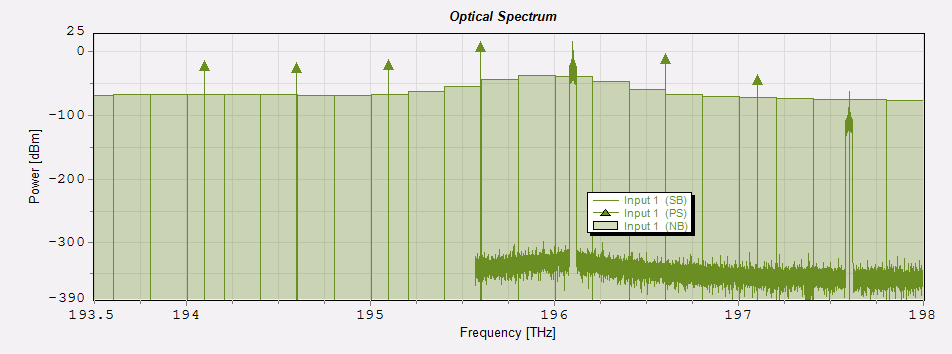
\includegraphics[width=11cm]{es7.png}\\
   \caption{Optical spectrum.}
   \label{es7}
\end{figure}

Channel 5, that corresponds to a frequency of 196.1 THz, now has a power of 19.356 dBm, while the channel 8,
corresponding to a frequency of 197.6 THz, has a power of -59.735 dBm.
The channel 5 increased its power, while channel 8 has a very low power, that is comparable to the power of the noise.
Now the difference between the two channels is about 79 dBm.

\newpage
%%%%%%%%%%%%%%%%%%%%%%%%%%%%%%%%%%%%%%%%%%%%%%%%%%%%%%%%%%%%%%%%%%%%%%%%%%%%%%%%%%%%%%%%%%%%%
\section*{Question 8}
Degradation of channel 8 is severe: the wavelength of the signal corresponding to this channel, in fact, is located in a
point of the gain curve of the amplifier where the gain is low.
At each loop the signal in this channel is attenuated and this is why at the end of simulation we obtain a so small power value.

%%%%%%%%%%%%%%%%%%%%%%%%%%%%%%%%%%%%%%%%%%%%%%%%%%%%%%%%%%%%%%%%%%%%%%%%%%%%%%%%%%%%%%%%%%%%%
\section*{Exercise 5}
We set the fiber length to 30 Km with 12 loops, and we measure the BER of all channels at various distances.
In Figure \ref{es5} is shown the result, in Figure \ref{es5zoom} is shown a zoom of the same graph.
We can observe that for distances higher than $\approx 11.6$ Km, the BER becomes unacceptable.

\begin{figure}[!ht]
   \centering
   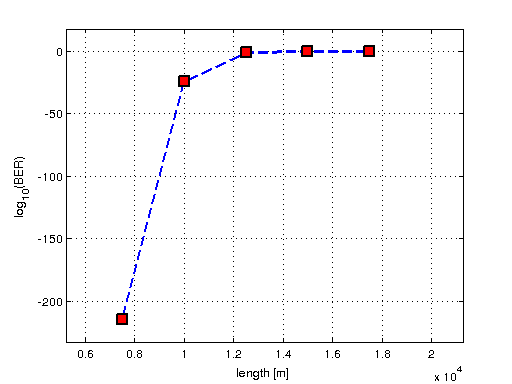
\includegraphics[width=11cm]{es5.png}\\
   \caption{BER versus length.}
   \label{es5}
\end{figure}

\begin{figure}[!ht]
   \centering
   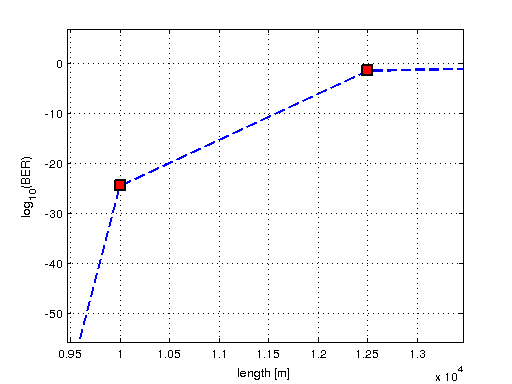
\includegraphics[width=11cm]{es5zoom.png}\\
   \caption{BER versus length (zoom).}
   \label{es5zoom}
\end{figure}


\newpage
%%%%%%%%%%%%%%%%%%%%%%%%%%%%%%%%%%%%%%%%%%%%%%%%%%%%%%%%%%%%%%%%%%%%%%%%%%%%%%%%%%%%%%%%%%%%%
\section*{Exercise 6}
We now vary the power of all the channels from 0 dBm to 12 dBm, in steps of 3 dBm.
In Figure \ref{exercise6} is shown the result, while in Figure \ref{exercise6zoom} is shown a zoom of the graph around the region of interest.
We can observe that, increasing the power of all the channels, the maximum distance that can be reached increases.
The maximum distances reachable within an acceptable BER, are nearly:
\begin{itemize}
 \item 0 dBm $\rightarrow$ $1.17 \cdot 10^4$ m
 \item 3 dBm $\rightarrow$ $1.205 \cdot 10^4$ m
 \item 6 dBm $\rightarrow$ $1.23 \cdot 10^4$ m
 \item 9 dBm $\rightarrow$ $1.245 \cdot 10^4$ m
 \item 12 dBm $\rightarrow$ $1.275 \cdot 10^4$ m
\end{itemize}


\begin{figure}[!ht]
   \centering
   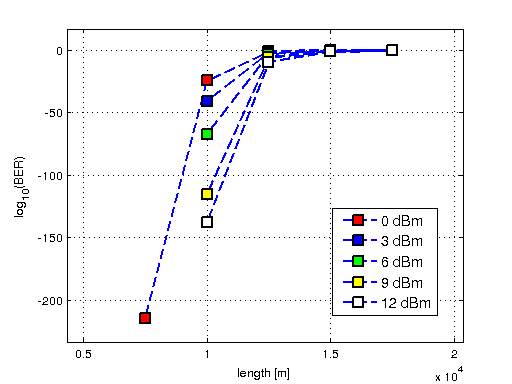
\includegraphics[width=11cm]{exercise6.png}\\
   \caption{BER versus length for different powers.}
   \label{exercise6}
\end{figure}

\begin{figure}[!ht]
   \centering
   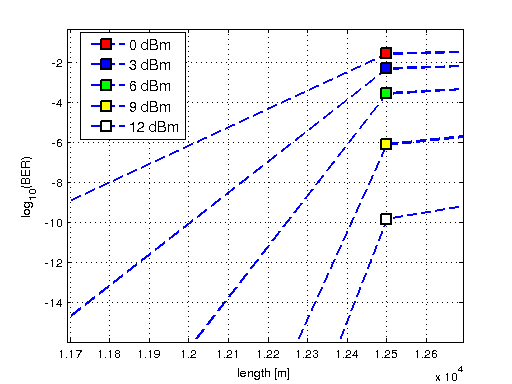
\includegraphics[width=11cm]{exercise6zoom.png}\\
   \caption{BER versus length for different powers (zoom).}
   \label{exercise6zoom}
\end{figure}


\newpage
%%%%%%%%%%%%%%%%%%%%%%%%%%%%%%%%%%%%%%%%%%%%%%%%%%%%%%%%%%%%%%%%%%%%%%%%%%%%%%%%%%%%%%%%%%%%%
\section*{Question 9}
EDFA amplifiers have non flat gain profile and we have seen that this is a critical problem in WDM systems with cascades of amplifiers:
in fact, small differences of gain become big power differences at the output.
Two techniques to obtain a flat gain are:
\begin{itemize}
 \item Pre-equalization
 \item Equalization
\end{itemize}

With pre-equalization we vary the transmitted power according to the gain: low where the gain is high and vice-versa.
This way tries to achieve the same power for all the channels. The problem is that is not possible to vary too much the input power
and so this is difficult to implement in real networks.

The second technique, equalization, consists in equalizing the channels at each EDFA stage. Multichannel filters are used, the best
solutions are: integrate a filter with the appropriate response into the amplifier, use dielectric thin film filters or use cascades
of LPG (Long Period Grating) filters.







\end{document}